\section{Modelado de Robots}
Ahora veremos cómo podemos construir y ver una visualización de un objeto en el programa rviz. Con eso, podremos construir una visualización de un robot.

Primero, creamos una carpeta llamada \texttt{urdf} dentro del paquete (justo debajo del paquete). Acá corregir, porque la imagen muestra que puse la carpeta en el espacio de trabajo y no en el paquete.

\begin{figure}[H] 
    \centering    
    \makebox[\textwidth][c]{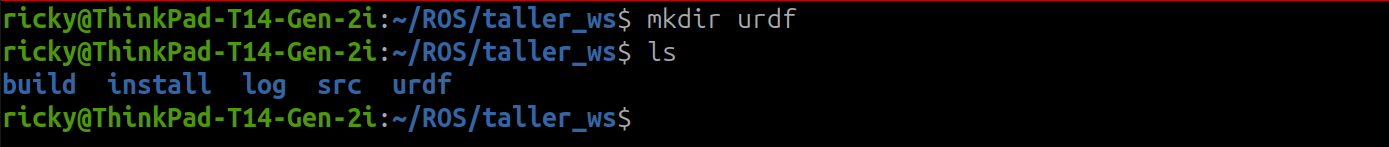
\includegraphics[width=1.4\textwidth]{imagenes/creacion-urdf.png}}
    \caption{Creación de carpeta urdf dentro del paquete.}
    \label{fig:mi_imagen}
\end{figure}

Ahora, vamos a crear un archivo \texttt{robot.urdf} dentro de la carpeta \texttt{urdf/}. \texttt{robot.urdf} contendrá lo siguiente:

\begin{center}
    \begin{Verbatim}[gobble=4]
    <?xml version="1.0"?>
    <robot name="paquito">
        <link name="base_link">
            <visual>
                <geometry>
                    <cylinder length="0.6" radius="0.2"/>
                </geometry>
                <material name="blue"><color rgba="0 0 .8 1"/></material>
            </visual>

            <collision>
                <geometry>
                    <cylinder length="0.6" radius="0.2"/>
                </geometry>
            </collision>
        </link>
    </robot>
    \end{Verbatim}
\end{center}

\begin{figure}[H] 
    \centering    
    \makebox[\textwidth][c]{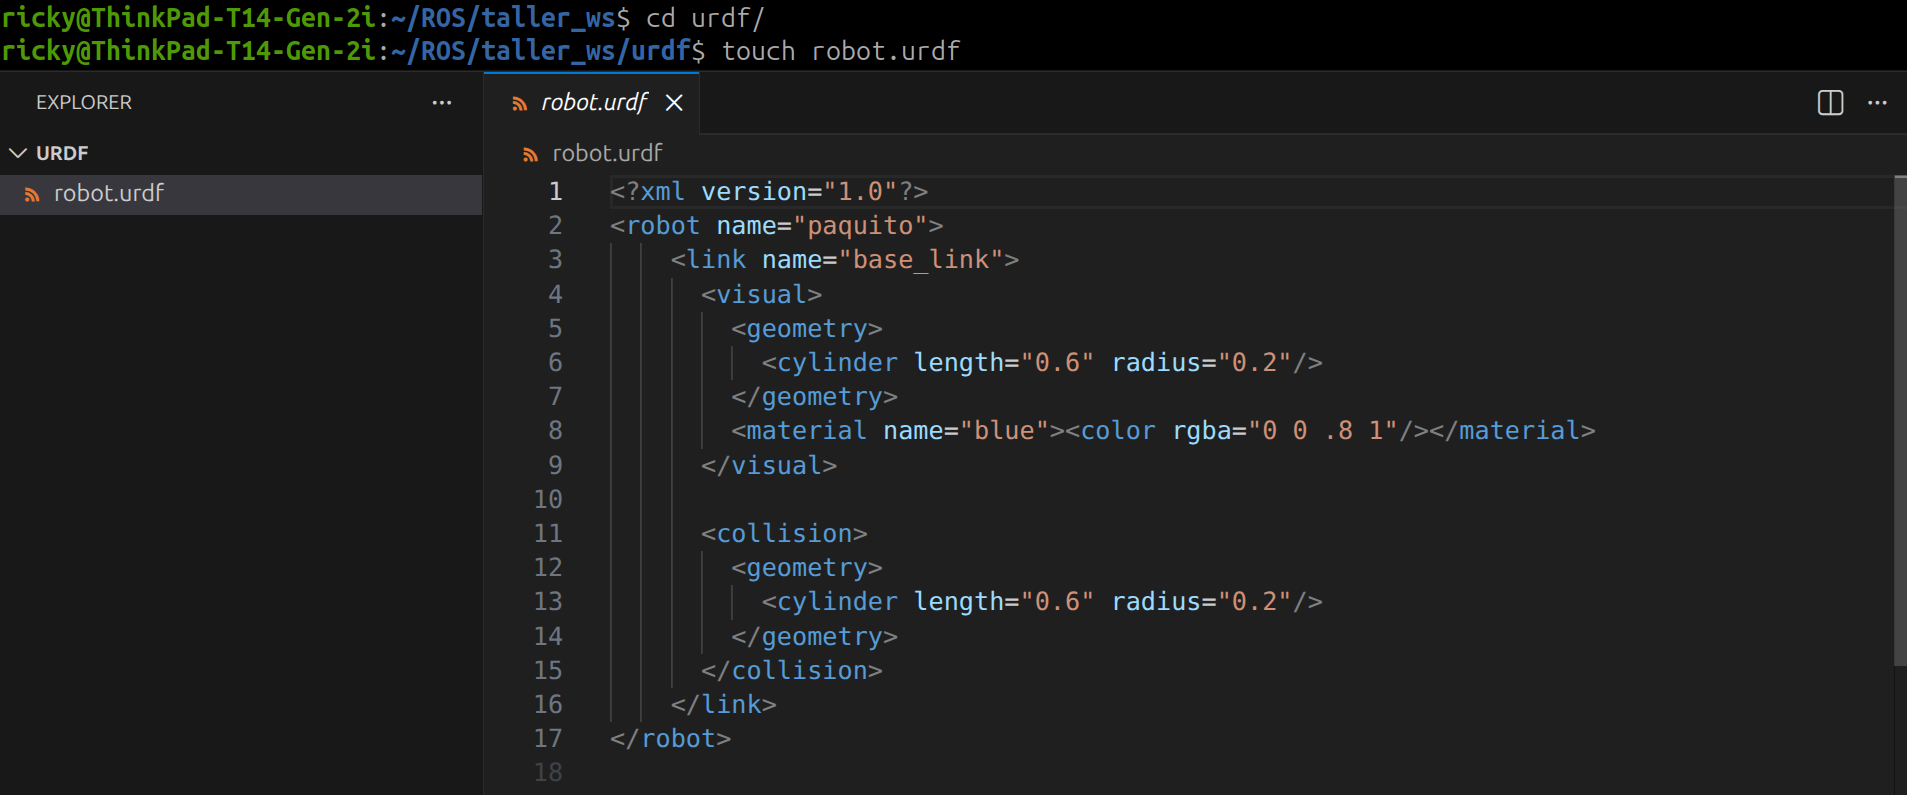
\includegraphics[width=1.4\textwidth]{imagenes/urdf2-3.png}}
    \caption{Creación de archivo robot.urdf.}
    \label{fig:mi_imagen}
\end{figure}

Luego, modificamos la línea \texttt{urdf} a la directiva install en el archivo \texttt{CMakeLists.txt}. La directiva install debe quedar como sigue:

\begin{center}
    \begin{Verbatim}[gobble=4]
        install (DIRECTORY
        launch 
        urdf # nueva línea
        DESTINATION share/${PROJECT_NAME}
        )
    \end{Verbatim}
\end{center}

\begin{figure}[H] 
    \centering    
    \makebox[\textwidth][c]{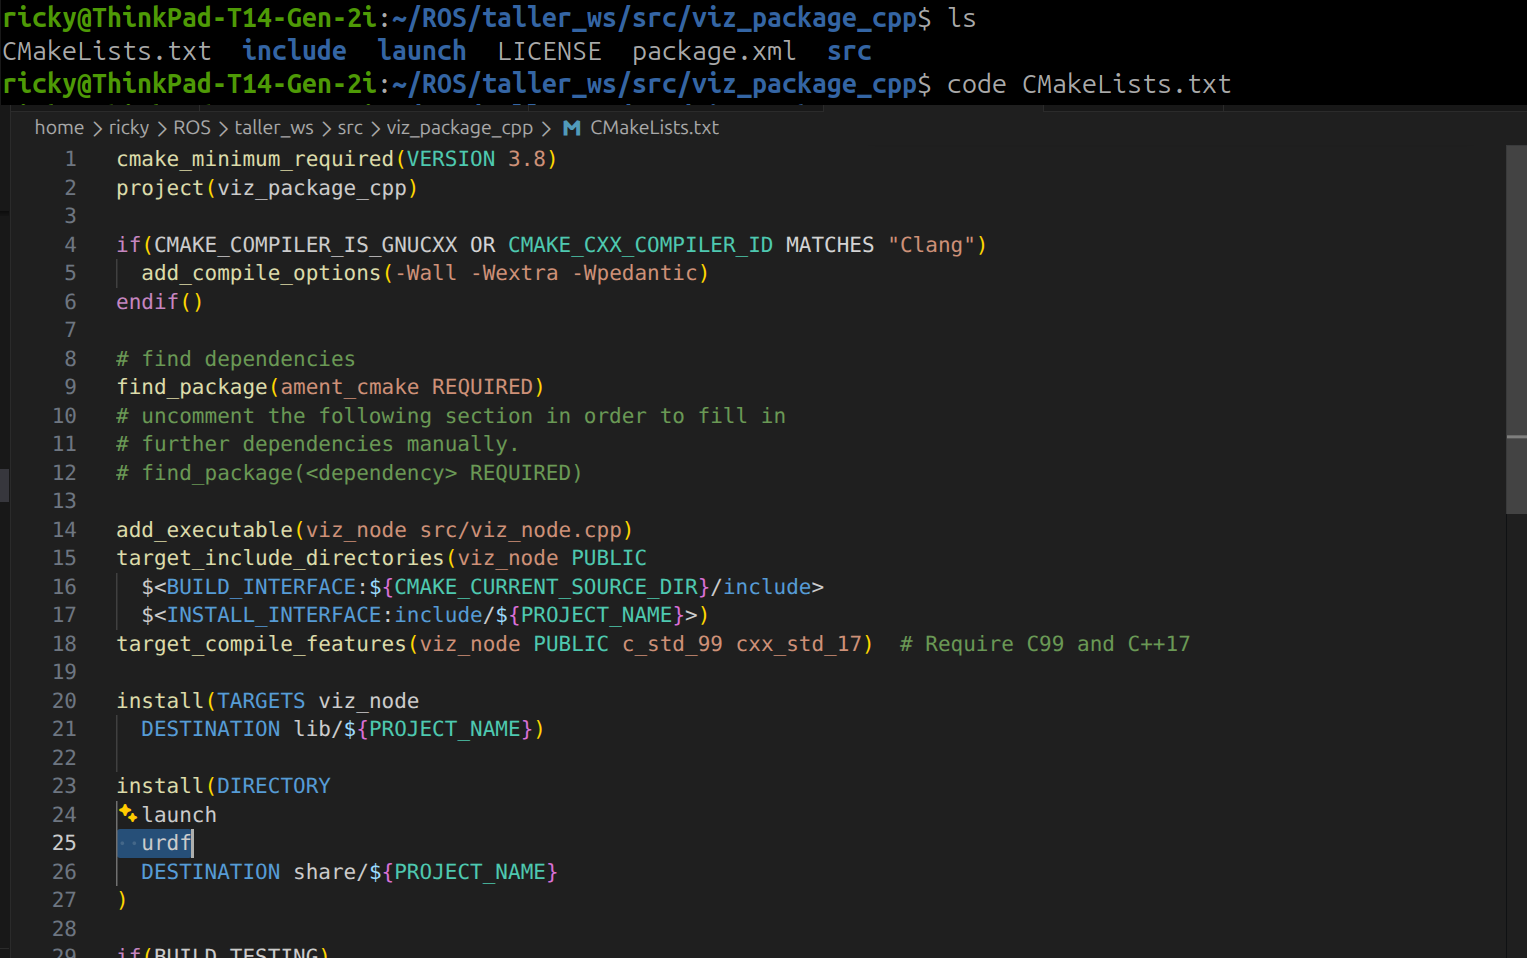
\includegraphics[width=1.4\textwidth]{imagenes/cmake-urdf3.png}}
    \caption{Agregar urdf a la directiva install del CMakeLists.txt.}
    \label{fig:mi_imagen}
\end{figure}

Ahora que ya tenemos la descripción de la forma del objeto a visualizar, pasaremos a la parte del movimiento. En el archivo \texttt{package.xml} del paquete, agregamos las siguientes líneas:

\begin{center}
    \begin{Verbatim}[gobble=4]
        <exec_depend>joint_state_publisher</exec_depend>
        <exec_depend>robot_state_publisher</exec_depend>
    \end{Verbatim}
\end{center}

\begin{figure}[H] 
    \centering    
    \makebox[\textwidth][c]{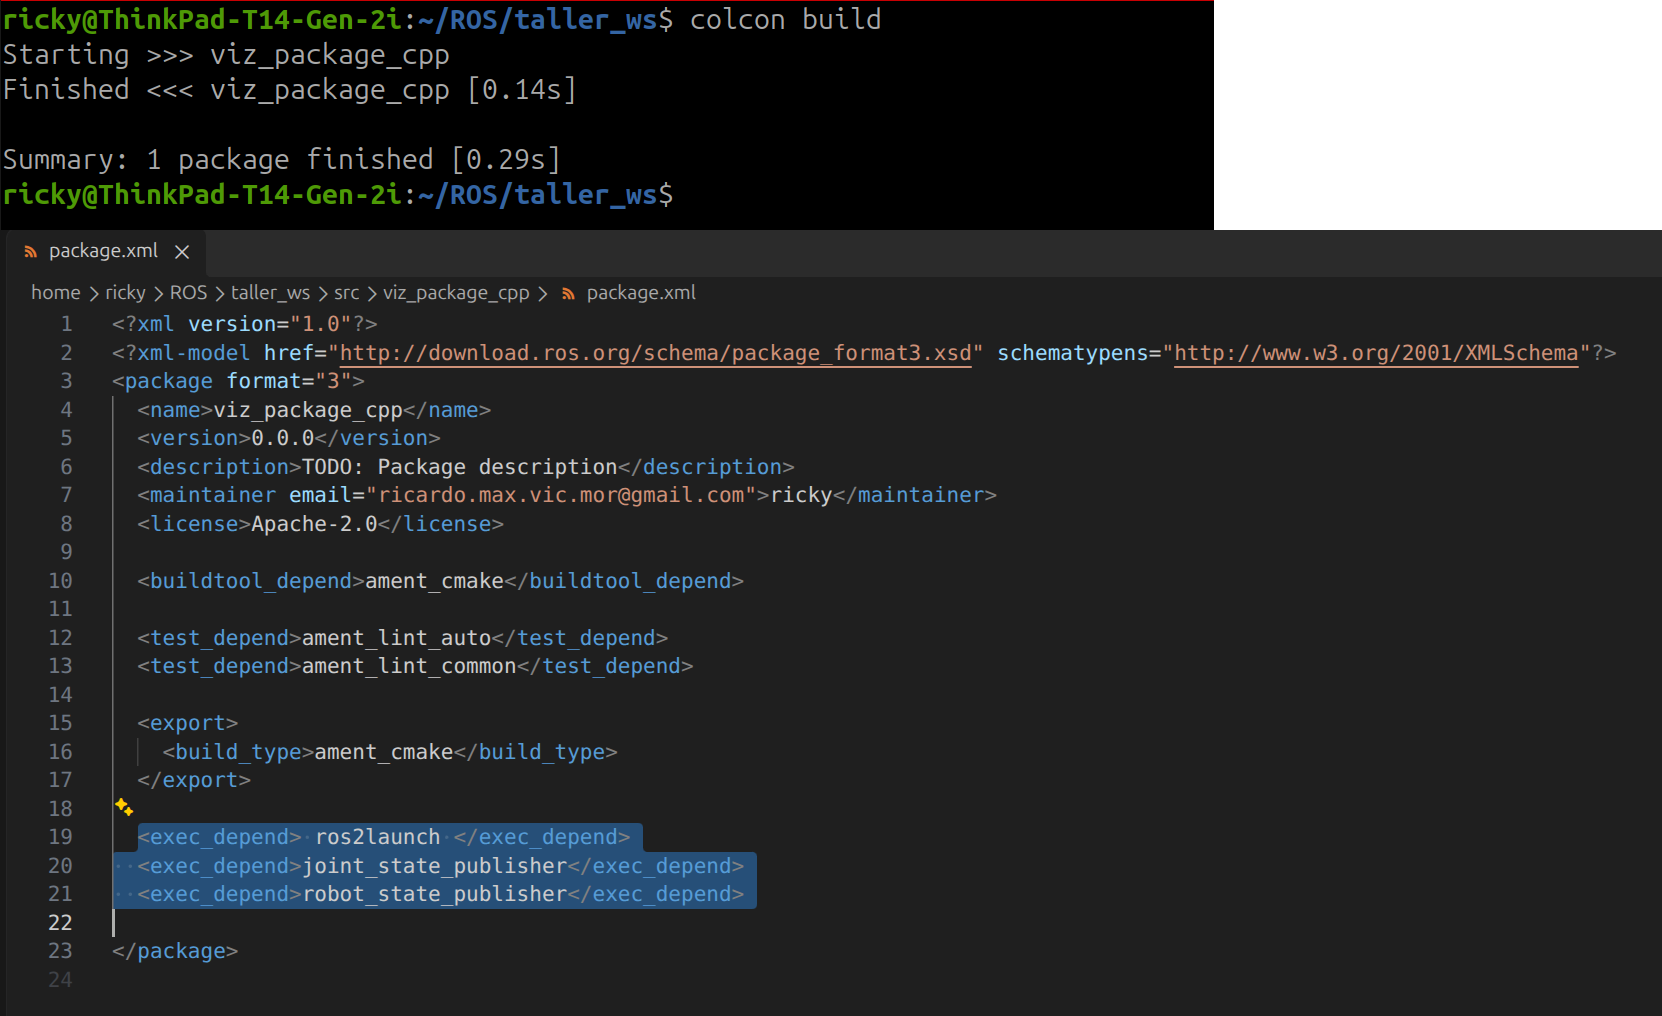
\includegraphics[width=1.4\textwidth]{imagenes/cmake52.png}}
    \caption{Modificación package.xml.}
    \label{fig:mi_imagen}
\end{figure}

Ejecutar el siguiente comando en el espacio de trabajo:

\begin{center}
    \begin{Verbatim}[gobble=4]
        rosdep install -i --from-path src --rosdistro jazzy -y        
    \end{Verbatim}
\end{center}

Si pide inicializar, ejecutar los comandos siguientes antes de ejecutar el comando anterior:

\begin{center}
    \begin{Verbatim}[gobble=4]
        sudo rosdep init
        rosdep update
    \end{Verbatim}
\end{center}


\begin{figure}[H] 
    \centering    
    \makebox[\textwidth][c]{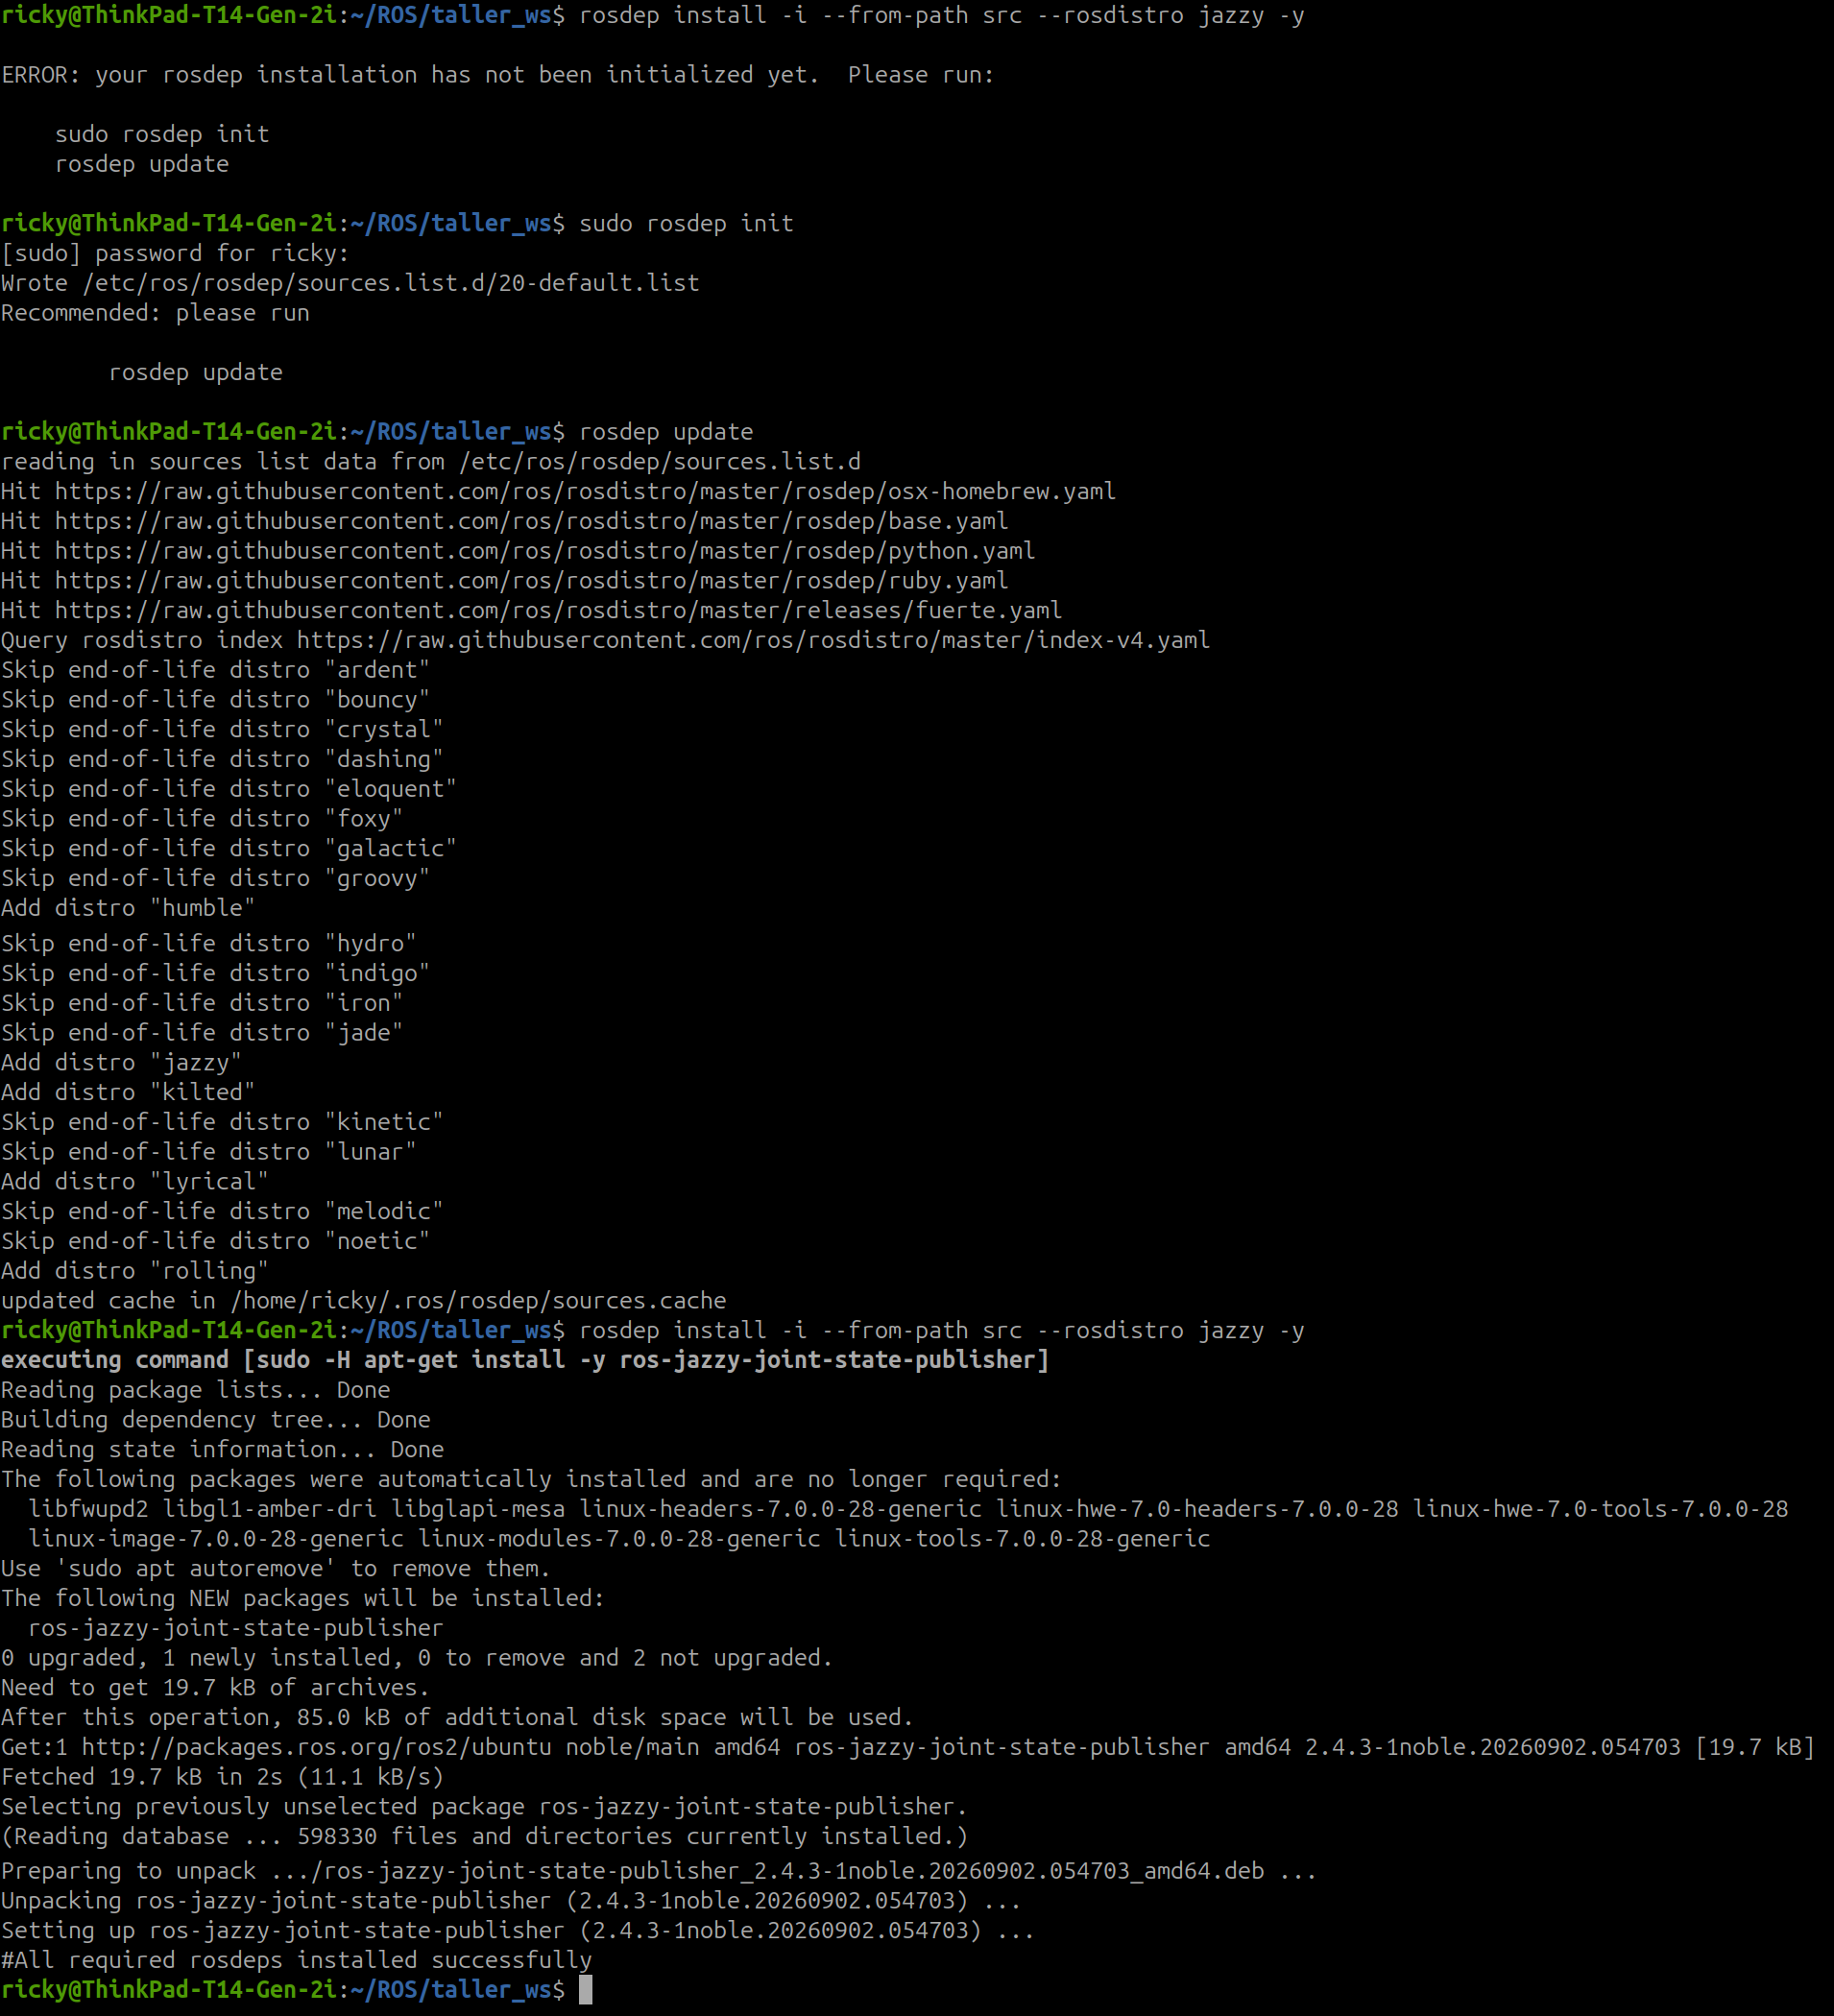
\includegraphics[width=1.4\textwidth]{imagenes/r123.png}}
    \caption{Instalación con rosdep.}
    \label{fig:mi_imagen}
\end{figure}

Ahora, hay que pedir al archivo de lanzamiento que ejecute al nodo que publicará la
descripción del robot. Modificamos al archivo \texttt{viz\_launch.py} para que quede de la siguiente forma.

\begin{center}
    \begin{Verbatim}[gobble=4]
        import os
        from ament_index_python.packages import get_package_share_directory
        from launch import LaunchDescription
        from launch_ros.actions import Node        
        
        def generate_launch_description():
        package_dir = get_package_share_directory('viz_package_cpp')
        path_to_urdf = os.path.join(package_dir, 'urdf', 'robot.urdf')
        
        with open(path_to_urdf, 'r') as f:
        robot_desc = f.read()
        
        return LaunchDescription([
            Node(
                package='viz_package_cpp',
                namespace='paquito1',
                executable='viz_node',
                name='viz',
                output='screen',
                ),
                Node(
                    package='robot_state_publisher',
                    name='robot_state_publisher',
                    executable='robot_state_publisher',
                    output='screen',
                    parameters=[{
                        'robot_description': robot_desc,
                        'publish_frequency': 30.0,
                        }]
                        )
                        ])
                        
                    \end{Verbatim}
                \end{center}
                
                
\begin{figure}[H] 
    \centering    
    \makebox[\textwidth][c]{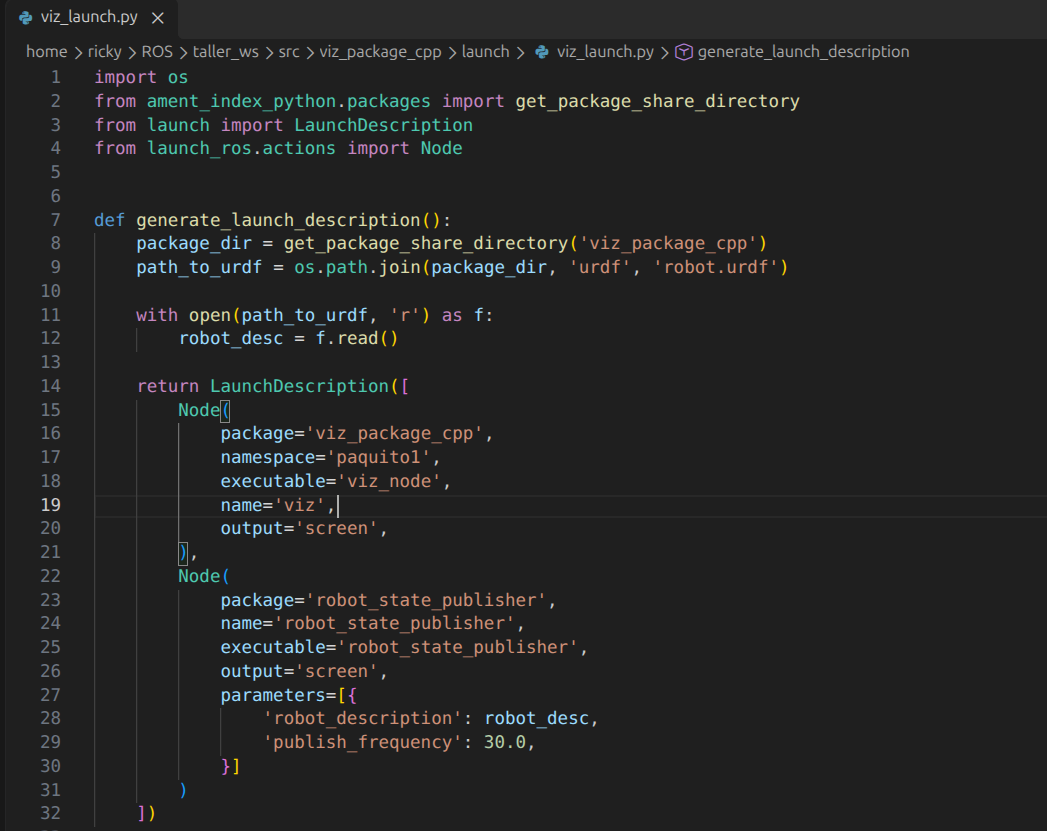
\includegraphics[width=1.4\textwidth]{imagenes/l2.png}}
    \caption{Modificación al launch file para publicar la figura.}
    \label{fig:mi_imagen}
\end{figure}
                
Ahora procedemos a compilar y lanzar el launchfile. Recordemos que esto se hace con los siguientes comandos y como sigue:                
                
\begin{center}
    \begin{Verbatim}[gobble=4]
    colcon build
    ros2 launch viz_package_cpp viz_launch.py
    \end{Verbatim}
\end{center}

\begin{figure}[H] 
    \centering    
    \makebox[\textwidth][c]{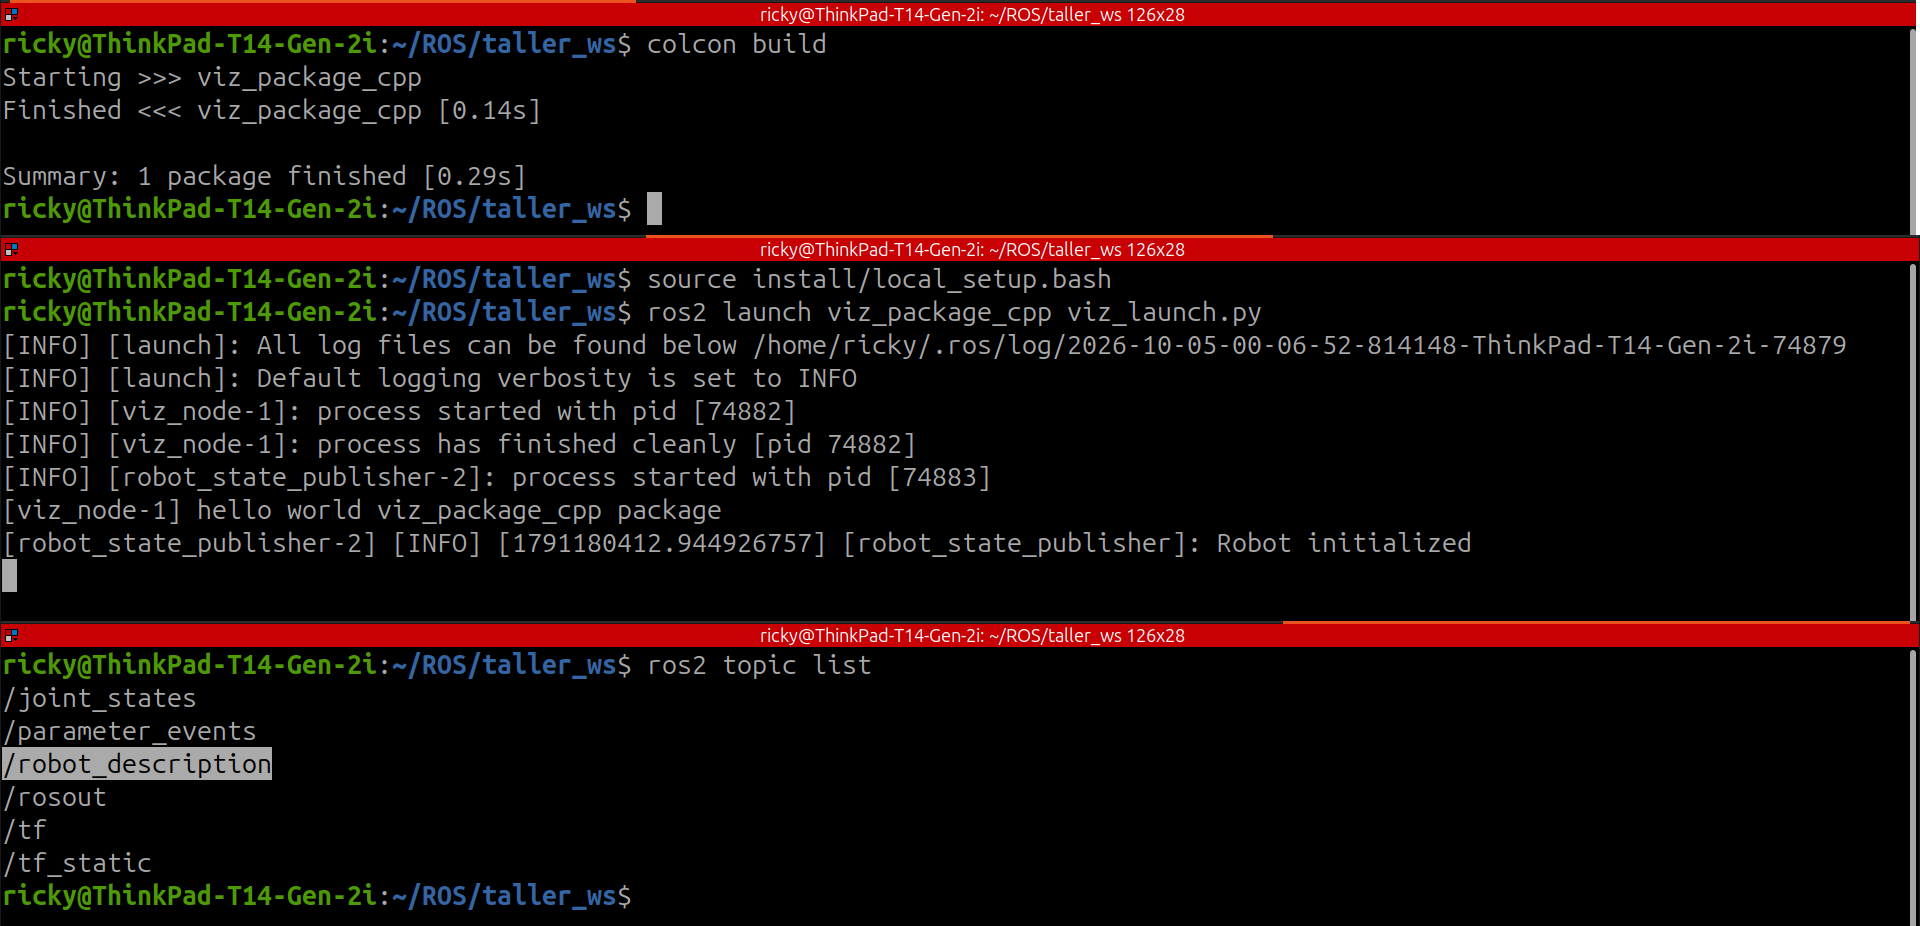
\includegraphics[width=1.4\textwidth]{imagenes/rdesc123.png}}
    \caption{Compilación, lanzamiento de launch file y listado de tópicos.}
    \label{fig:mi_imagen}
\end{figure}

Vemos de la figura anterior, en la terminal 2, que se sigue ejecutando el nodo de hola mundo, y además se ejecuta el segundo nodo que publica la descripción del robot. Podemos comprobar que se publica la descripción del robot en la terminal 3, porque se publica el tópico \texttt{/robot\_description}.





